\documentclass[10pt,a4paper]{article}
\usepackage[utf8]{inputenc}
\usepackage{amsmath}
\usepackage{amsfonts}
\usepackage{amssymb}
\usepackage{graphicx}
\usepackage[margin=0.5in]{geometry}

\author{Oleg Loshkin}
\title{\textbf{UPDC}\\Unity to PokEngine Data Converter\\\textbf{User Manual}}
\graphicspath{{./images/}}

\begin{document}
\maketitle
\section{Introduction}
The \textbf{Unity to PokEngine Data Converter, or UPDC for short}, is a Unity tool used to \textbf{export ScriptableObject} inheriting .asset files \textbf{into JSON files} that end with extensions that specify their type. These JSON files can then be read by the PokEngine's parser.

\section{Accessing the Tool}
\begin{center}
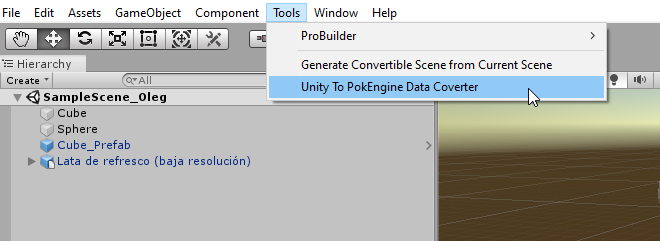
\includegraphics[scale=1.0]{mainMenu}
\end{center}

\section{Folder Hierarchy}
\begin{center}
\includegraphics[scale=0.425]{folderUPDC}
\end{center}

\section{The Exporter Tab}
\begin{center}
\includegraphics[scale=0.55]{exportUi}
\end{center}
The tool is separated between \textbf{two tabs}. In the \textbf{Exporter tab}, you can \textbf{select the .asset files located in the Assets/Data/...} folders \textbf{you wish to export}.
You can \textbf{select the output directory} for the files generated. By default, the tool outputs the files into Assets/Editor/UPDC/DefaultOutputDir you have previously defined.
Upon exportation, \textbf{directories will be generated in the output directory} to mirror the structure seen in Assets/Data.\\
Finally, you can choose whether to \textbf{overwrite any existing files} or not.
\newpage

\section{Integrating with UPDC}
\textbf{UPDC converts .asset files} of types \textbf{inheriting from the ScriptableObject} class.\\
If you wish to export your data using UPDC, you will therefore need to \textbf{create your ScriptableObject inheriting class} as such:
\begin{center}
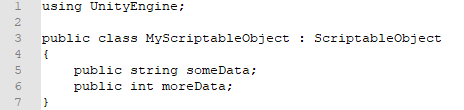
\includegraphics[scale=1.0]{soExample}
\end{center}
\textbf{Instances of your ScriptableObject inheriting class will need to be stored in Asssets/Data/yourTypeFolder} for UPDC to manage them. \textbf{This must be done on your side} as UPDC does not provide any automatic way to put your .asset files into their corresponding folders.
Next, you will need to \textbf{define your new class with UPDC} via the "Types" tab.

\section{The Types Tab}
\begin{center}
\includegraphics[scale=0.55]{typesUi}
\end{center}
The \textbf{Types tab} contains a list of \textbf{tuples that define a type's name and it's corresponding extension}.
The type's name is used for generating appropriately named folders and the extension is appended to the JSONs generated for your custom class to be used by the PokEngine's parser to identify the asset's type.
\textbf{To integrate your newly created class} with UPDC, simply \textbf{enter it's name and it's extension} in the "New entry" fields and press the \textbf{"Add new type" button}.
A \textbf{folder for your new .asset files will be automatically generated} in Assets/Data and the files will be visible in the "Export" tab.\\
To \textbf{remove a type}, simply \textbf{select it} in the list and press the \textbf{"Remove selected" button}.

\section{The Empty Fields Tab}
Unity's \textbf{JSONUtility} used for exporting ScriptableObjects \textbf{fills any uninitialized fields} of a ScriptableObject \textbf{with default empty values}. This adds a lot of \textbf{useless contents in the output JSON file}. \textbf{UPDC therefore removes those} empty fields before writing the final version of the JSON to disk.\\
The \textbf{tool does however need to know what an empty field looks like}. If you don't want your JSON file to contain empty fields, \textbf{add a new definition of the string to be removed} from the resulting JSON like so:
\begin{center}
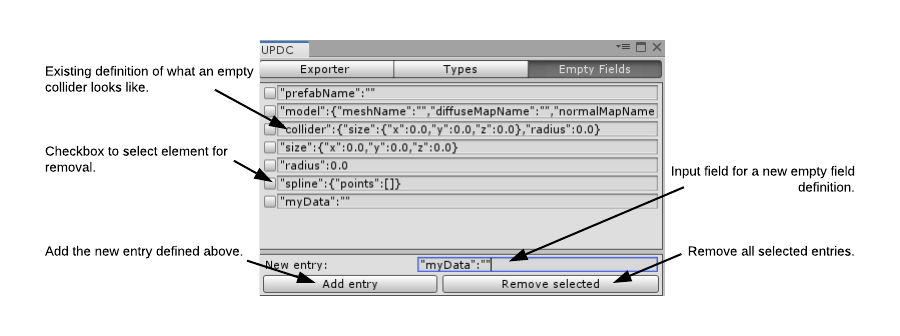
\includegraphics[scale=0.6]{EmptyFieldsUI}
\end{center}
This results in a JSON file containing only the initialized values like so:
\begin{center}
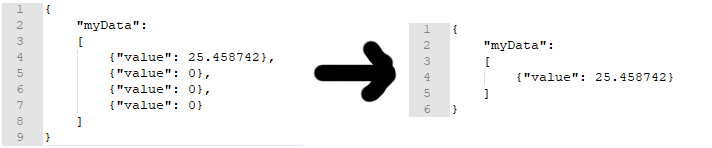
\includegraphics[scale=1.0]{cleaningJson}
\end{center}

\end{document}
